% Options for packages loaded elsewhere
\PassOptionsToPackage{unicode}{hyperref}
\PassOptionsToPackage{hyphens}{url}
\PassOptionsToPackage{dvipsnames,svgnames,x11names}{xcolor}
%
\documentclass[
  letterpaper,
  DIV=11,
  numbers=noendperiod]{scrartcl}

\usepackage{amsmath,amssymb}
\usepackage{lmodern}
\usepackage{iftex}
\ifPDFTeX
  \usepackage[T1]{fontenc}
  \usepackage[utf8]{inputenc}
  \usepackage{textcomp} % provide euro and other symbols
\else % if luatex or xetex
  \usepackage{unicode-math}
  \defaultfontfeatures{Scale=MatchLowercase}
  \defaultfontfeatures[\rmfamily]{Ligatures=TeX,Scale=1}
\fi
% Use upquote if available, for straight quotes in verbatim environments
\IfFileExists{upquote.sty}{\usepackage{upquote}}{}
\IfFileExists{microtype.sty}{% use microtype if available
  \usepackage[]{microtype}
  \UseMicrotypeSet[protrusion]{basicmath} % disable protrusion for tt fonts
}{}
\makeatletter
\@ifundefined{KOMAClassName}{% if non-KOMA class
  \IfFileExists{parskip.sty}{%
    \usepackage{parskip}
  }{% else
    \setlength{\parindent}{0pt}
    \setlength{\parskip}{6pt plus 2pt minus 1pt}}
}{% if KOMA class
  \KOMAoptions{parskip=half}}
\makeatother
\usepackage{xcolor}
\setlength{\emergencystretch}{3em} % prevent overfull lines
\setcounter{secnumdepth}{-\maxdimen} % remove section numbering
% Make \paragraph and \subparagraph free-standing
\ifx\paragraph\undefined\else
  \let\oldparagraph\paragraph
  \renewcommand{\paragraph}[1]{\oldparagraph{#1}\mbox{}}
\fi
\ifx\subparagraph\undefined\else
  \let\oldsubparagraph\subparagraph
  \renewcommand{\subparagraph}[1]{\oldsubparagraph{#1}\mbox{}}
\fi

\usepackage{color}
\usepackage{fancyvrb}
\newcommand{\VerbBar}{|}
\newcommand{\VERB}{\Verb[commandchars=\\\{\}]}
\DefineVerbatimEnvironment{Highlighting}{Verbatim}{commandchars=\\\{\}}
% Add ',fontsize=\small' for more characters per line
\usepackage{framed}
\definecolor{shadecolor}{RGB}{241,243,245}
\newenvironment{Shaded}{\begin{snugshade}}{\end{snugshade}}
\newcommand{\AlertTok}[1]{\textcolor[rgb]{0.68,0.00,0.00}{#1}}
\newcommand{\AnnotationTok}[1]{\textcolor[rgb]{0.37,0.37,0.37}{#1}}
\newcommand{\AttributeTok}[1]{\textcolor[rgb]{0.40,0.45,0.13}{#1}}
\newcommand{\BaseNTok}[1]{\textcolor[rgb]{0.68,0.00,0.00}{#1}}
\newcommand{\BuiltInTok}[1]{\textcolor[rgb]{0.00,0.23,0.31}{#1}}
\newcommand{\CharTok}[1]{\textcolor[rgb]{0.13,0.47,0.30}{#1}}
\newcommand{\CommentTok}[1]{\textcolor[rgb]{0.37,0.37,0.37}{#1}}
\newcommand{\CommentVarTok}[1]{\textcolor[rgb]{0.37,0.37,0.37}{\textit{#1}}}
\newcommand{\ConstantTok}[1]{\textcolor[rgb]{0.56,0.35,0.01}{#1}}
\newcommand{\ControlFlowTok}[1]{\textcolor[rgb]{0.00,0.23,0.31}{#1}}
\newcommand{\DataTypeTok}[1]{\textcolor[rgb]{0.68,0.00,0.00}{#1}}
\newcommand{\DecValTok}[1]{\textcolor[rgb]{0.68,0.00,0.00}{#1}}
\newcommand{\DocumentationTok}[1]{\textcolor[rgb]{0.37,0.37,0.37}{\textit{#1}}}
\newcommand{\ErrorTok}[1]{\textcolor[rgb]{0.68,0.00,0.00}{#1}}
\newcommand{\ExtensionTok}[1]{\textcolor[rgb]{0.00,0.23,0.31}{#1}}
\newcommand{\FloatTok}[1]{\textcolor[rgb]{0.68,0.00,0.00}{#1}}
\newcommand{\FunctionTok}[1]{\textcolor[rgb]{0.28,0.35,0.67}{#1}}
\newcommand{\ImportTok}[1]{\textcolor[rgb]{0.00,0.46,0.62}{#1}}
\newcommand{\InformationTok}[1]{\textcolor[rgb]{0.37,0.37,0.37}{#1}}
\newcommand{\KeywordTok}[1]{\textcolor[rgb]{0.00,0.23,0.31}{#1}}
\newcommand{\NormalTok}[1]{\textcolor[rgb]{0.00,0.23,0.31}{#1}}
\newcommand{\OperatorTok}[1]{\textcolor[rgb]{0.37,0.37,0.37}{#1}}
\newcommand{\OtherTok}[1]{\textcolor[rgb]{0.00,0.23,0.31}{#1}}
\newcommand{\PreprocessorTok}[1]{\textcolor[rgb]{0.68,0.00,0.00}{#1}}
\newcommand{\RegionMarkerTok}[1]{\textcolor[rgb]{0.00,0.23,0.31}{#1}}
\newcommand{\SpecialCharTok}[1]{\textcolor[rgb]{0.37,0.37,0.37}{#1}}
\newcommand{\SpecialStringTok}[1]{\textcolor[rgb]{0.13,0.47,0.30}{#1}}
\newcommand{\StringTok}[1]{\textcolor[rgb]{0.13,0.47,0.30}{#1}}
\newcommand{\VariableTok}[1]{\textcolor[rgb]{0.07,0.07,0.07}{#1}}
\newcommand{\VerbatimStringTok}[1]{\textcolor[rgb]{0.13,0.47,0.30}{#1}}
\newcommand{\WarningTok}[1]{\textcolor[rgb]{0.37,0.37,0.37}{\textit{#1}}}

\providecommand{\tightlist}{%
  \setlength{\itemsep}{0pt}\setlength{\parskip}{0pt}}\usepackage{longtable,booktabs,array}
\usepackage{calc} % for calculating minipage widths
% Correct order of tables after \paragraph or \subparagraph
\usepackage{etoolbox}
\makeatletter
\patchcmd\longtable{\par}{\if@noskipsec\mbox{}\fi\par}{}{}
\makeatother
% Allow footnotes in longtable head/foot
\IfFileExists{footnotehyper.sty}{\usepackage{footnotehyper}}{\usepackage{footnote}}
\makesavenoteenv{longtable}
\usepackage{graphicx}
\makeatletter
\def\maxwidth{\ifdim\Gin@nat@width>\linewidth\linewidth\else\Gin@nat@width\fi}
\def\maxheight{\ifdim\Gin@nat@height>\textheight\textheight\else\Gin@nat@height\fi}
\makeatother
% Scale images if necessary, so that they will not overflow the page
% margins by default, and it is still possible to overwrite the defaults
% using explicit options in \includegraphics[width, height, ...]{}
\setkeys{Gin}{width=\maxwidth,height=\maxheight,keepaspectratio}
% Set default figure placement to htbp
\makeatletter
\def\fps@figure{htbp}
\makeatother

\KOMAoption{captions}{tableheading}
\makeatletter
\makeatother
\makeatletter
\makeatother
\makeatletter
\@ifpackageloaded{caption}{}{\usepackage{caption}}
\AtBeginDocument{%
\ifdefined\contentsname
  \renewcommand*\contentsname{Table of contents}
\else
  \newcommand\contentsname{Table of contents}
\fi
\ifdefined\listfigurename
  \renewcommand*\listfigurename{List of Figures}
\else
  \newcommand\listfigurename{List of Figures}
\fi
\ifdefined\listtablename
  \renewcommand*\listtablename{List of Tables}
\else
  \newcommand\listtablename{List of Tables}
\fi
\ifdefined\figurename
  \renewcommand*\figurename{Figure}
\else
  \newcommand\figurename{Figure}
\fi
\ifdefined\tablename
  \renewcommand*\tablename{Table}
\else
  \newcommand\tablename{Table}
\fi
}
\@ifpackageloaded{float}{}{\usepackage{float}}
\floatstyle{ruled}
\@ifundefined{c@chapter}{\newfloat{codelisting}{h}{lop}}{\newfloat{codelisting}{h}{lop}[chapter]}
\floatname{codelisting}{Listing}
\newcommand*\listoflistings{\listof{codelisting}{List of Listings}}
\makeatother
\makeatletter
\@ifpackageloaded{caption}{}{\usepackage{caption}}
\@ifpackageloaded{subcaption}{}{\usepackage{subcaption}}
\makeatother
\makeatletter
\@ifpackageloaded{tcolorbox}{}{\usepackage[many]{tcolorbox}}
\makeatother
\makeatletter
\@ifundefined{shadecolor}{\definecolor{shadecolor}{rgb}{.97, .97, .97}}
\makeatother
\makeatletter
\makeatother
\ifLuaTeX
  \usepackage{selnolig}  % disable illegal ligatures
\fi
\IfFileExists{bookmark.sty}{\usepackage{bookmark}}{\usepackage{hyperref}}
\IfFileExists{xurl.sty}{\usepackage{xurl}}{} % add URL line breaks if available
\urlstyle{same} % disable monospaced font for URLs
\hypersetup{
  colorlinks=true,
  linkcolor={blue},
  filecolor={Maroon},
  citecolor={Blue},
  urlcolor={Blue},
  pdfcreator={LaTeX via pandoc}}

\author{}
\date{}

\begin{document}
\ifdefined\Shaded\renewenvironment{Shaded}{\begin{tcolorbox}[borderline west={3pt}{0pt}{shadecolor}, interior hidden, sharp corners, breakable, boxrule=0pt, frame hidden, enhanced]}{\end{tcolorbox}}\fi

::: \{.cell \_cell\_guid=`b1076dfc-b9ad-4769-8c92-a6c4dae69d19'
\_uuid=`8f2839f25d086af736a60e9eeb907d3b93b6e0e5'
execution=`\{``iopub.execute\_input'':``2023-05-18T13:45:05.122442Z'',``iopub.status.busy'':``2023-05-18T13:45:05.122109Z'',``iopub.status.idle'':``2023-05-18T13:45:05.152481Z'',``shell.execute\_reply'':``2023-05-18T13:45:05.151239Z'',``shell.execute\_reply.started'':``2023-05-18T13:45:05.122418Z''\}'
trusted=`true' execution\_count=1\}

\begin{Shaded}
\begin{Highlighting}[]
\ImportTok{import}\NormalTok{ numpy }\ImportTok{as}\NormalTok{ np }\CommentTok{\# linear algebra}
\ImportTok{import}\NormalTok{ pandas }\ImportTok{as}\NormalTok{ pd }\CommentTok{\# data processing, CSV file I/O (e.g. pd.read\_csv)}
\ImportTok{import}\NormalTok{ matplotlib.pyplot }\ImportTok{as}\NormalTok{ plt}
\ImportTok{import}\NormalTok{ os}
\ControlFlowTok{for}\NormalTok{ dirname, \_, filenames }\KeywordTok{in}\NormalTok{ os.walk(}\StringTok{\textquotesingle{}/kaggle/input\textquotesingle{}}\NormalTok{):}
    \ControlFlowTok{for}\NormalTok{ filename }\KeywordTok{in}\NormalTok{ filenames:}
        \BuiltInTok{print}\NormalTok{(os.path.join(dirname, filename))}
\end{Highlighting}
\end{Shaded}

\begin{verbatim}
/kaggle/input/transformer/DatasetB.csv
/kaggle/input/transformer/DatasetA.csv
\end{verbatim}

:::

Here, we have loaded the data and set Furan as the label. At first, we
have used 25 percent of the dataset A as the test set to come up with a
good model, and then use this model to test in the dataset B.

\begin{Shaded}
\begin{Highlighting}[]
\NormalTok{ds\_A }\OperatorTok{=}\NormalTok{ pd.read\_csv(}\StringTok{"/kaggle/input/transformer/DatasetA.csv"}\NormalTok{)}
\NormalTok{ds\_B }\OperatorTok{=}\NormalTok{ pd.read\_csv(}\StringTok{"/kaggle/input/transformer/DatasetB.csv"}\NormalTok{)}

\CommentTok{\# Splitting train and test}
\ImportTok{from}\NormalTok{ sklearn.model\_selection }\ImportTok{import}\NormalTok{ train\_test\_split}
\NormalTok{train\_set\_A, test\_set\_A }\OperatorTok{=}\NormalTok{ train\_test\_split(ds\_A, test\_size }\OperatorTok{=} \FloatTok{0.25}\NormalTok{, random\_state }\OperatorTok{=} \DecValTok{11}\NormalTok{)}

\CommentTok{\# Setting the labels}
\NormalTok{y\_train\_A }\OperatorTok{=}\NormalTok{ train\_set\_A[}\StringTok{\textquotesingle{}Furan\textquotesingle{}}\NormalTok{]}
\NormalTok{y\_test\_A }\OperatorTok{=}\NormalTok{ test\_set\_A[}\StringTok{\textquotesingle{}Furan\textquotesingle{}}\NormalTok{]}

\CommentTok{\# Dropping the Furan and Health Index columns}
\NormalTok{X\_train\_A }\OperatorTok{=}\NormalTok{ train\_set\_A.drop([}\StringTok{"Furan"}\NormalTok{, }\StringTok{"HI"}\NormalTok{], axis }\OperatorTok{=} \DecValTok{1}\NormalTok{)}
\NormalTok{X\_test\_A }\OperatorTok{=}\NormalTok{ test\_set\_A.drop([}\StringTok{"Furan"}\NormalTok{, }\StringTok{"HI"}\NormalTok{], axis }\OperatorTok{=} \DecValTok{1}\NormalTok{)}

\CommentTok{\# For DatasetB}
\NormalTok{y\_B }\OperatorTok{=}\NormalTok{ ds\_B[}\StringTok{\textquotesingle{}Furan\textquotesingle{}}\NormalTok{]}
\NormalTok{X\_B }\OperatorTok{=}\NormalTok{ ds\_B.drop([}\StringTok{"Furan"}\NormalTok{, }\StringTok{"HI"}\NormalTok{], axis }\OperatorTok{=} \DecValTok{1}\NormalTok{)}

\CommentTok{\# The code below is for the second case, where we train the data for the whole}
\CommentTok{\# Dataset A and test it on Dataset B}
\NormalTok{y\_A }\OperatorTok{=}\NormalTok{ ds\_A[}\StringTok{\textquotesingle{}Furan\textquotesingle{}}\NormalTok{]}
\NormalTok{X\_A }\OperatorTok{=}\NormalTok{ ds\_A.drop([}\StringTok{"Furan"}\NormalTok{, }\StringTok{"HI"}\NormalTok{], axis }\OperatorTok{=} \DecValTok{1}\NormalTok{)}
\end{Highlighting}
\end{Shaded}

\begin{verbatim}
/opt/conda/lib/python3.10/site-packages/scipy/__init__.py:146: UserWarning: A NumPy version >=1.16.5 and <1.23.0 is required for this version of SciPy (detected version 1.23.5
  warnings.warn(f"A NumPy version >={np_minversion} and <{np_maxversion}"
\end{verbatim}

The code below, drops the columns that we don't need, and only keeps the
common features between dataset A and B.

\begin{Shaded}
\begin{Highlighting}[]
\NormalTok{X\_train\_A }\OperatorTok{=}\NormalTok{ X\_train\_A.drop(}\BuiltInTok{set}\NormalTok{(ds\_A.columns) }\OperatorTok{{-}} \BuiltInTok{set}\NormalTok{(ds\_B.columns), axis}\OperatorTok{=}\DecValTok{1}\NormalTok{)}
\NormalTok{X\_test\_A }\OperatorTok{=}\NormalTok{ X\_test\_A.drop(}\BuiltInTok{set}\NormalTok{(ds\_A.columns) }\OperatorTok{{-}} \BuiltInTok{set}\NormalTok{(ds\_B.columns), axis}\OperatorTok{=}\DecValTok{1}\NormalTok{)}
\NormalTok{X\_A }\OperatorTok{=}\NormalTok{ X\_A.drop(}\BuiltInTok{set}\NormalTok{(ds\_A.columns) }\OperatorTok{{-}} \BuiltInTok{set}\NormalTok{(ds\_B.columns), axis}\OperatorTok{=}\DecValTok{1}\NormalTok{)}
\NormalTok{X\_B }\OperatorTok{=}\NormalTok{ X\_B[X\_train\_A.columns]}
\NormalTok{X\_train\_A}
\end{Highlighting}
\end{Shaded}

\begin{longtable}[]{@{}llllllllll@{}}
\toprule()
& H2 & Methane & Acetylene & Ethylene & Ethane & Water & Acid & BDV &
IFT \\
\midrule()
\endhead
109 & 12.2 & 53.50 & 6.9 & 127.4 & 48.0 & 3 & 0.043 & 83.0 & 20 \\
566 & 30.2 & 0.00 & 0.0 & 2.6 & 1.1 & 3 & 0.005 & 84.0 & 39 \\
410 & 45.6 & 18.20 & 0.0 & 1.6 & 1.7 & 5 & 0.005 & 87.0 & 30 \\
316 & 19.7 & 38.50 & 0.0 & 2.7 & 41.6 & 7 & 0.005 & 50.0 & 32 \\
678 & 11.0 & 7.60 & 0.0 & 0.3 & 1.6 & 3 & 0.005 & 61.0 & 42 \\
... & ... & ... & ... & ... & ... & ... & ... & ... & ... \\
269 & 13.7 & 5.10 & 0.0 & 0.4 & 1.1 & 1 & 0.005 & 94.0 & 36 \\
337 & 32.9 & 3.77 & 0.0 & 0.6 & 2.4 & 6 & 0.005 & 79.0 & 32 \\
91 & 22.8 & 3.30 & 0.0 & 4.9 & 3.0 & 11 & 0.140 & 88.0 & 16 \\
80 & 61.2 & 27.30 & 0.0 & 25.6 & 20.8 & 9 & 0.099 & 70.0 & 17 \\
703 & 58.1 & 9.40 & 0.0 & 1.4 & 1.9 & 5 & 0.005 & 86.0 & 33 \\
\bottomrule()
\end{longtable}

The code below, discretizes the Furan data into 3 classes.

\begin{Shaded}
\begin{Highlighting}[]
\CommentTok{\# define the bin edges for each class}
\NormalTok{bins }\OperatorTok{=}\NormalTok{ [}\OperatorTok{{-}}\DecValTok{1}\NormalTok{, }\FloatTok{0.1}\NormalTok{, }\DecValTok{1}\NormalTok{, }\DecValTok{100}\NormalTok{]}

\CommentTok{\# define the labels for each class}
\NormalTok{labels }\OperatorTok{=}\NormalTok{ [}\DecValTok{0}\NormalTok{, }\DecValTok{1}\NormalTok{, }\DecValTok{2}\NormalTok{]}

\NormalTok{y\_train\_A }\OperatorTok{=}\NormalTok{ pd.DataFrame(y\_train\_A)}
\NormalTok{y\_B }\OperatorTok{=}\NormalTok{ pd.DataFrame(y\_B)}
\NormalTok{y\_test\_A }\OperatorTok{=}\NormalTok{ pd.DataFrame(y\_test\_A)}
\NormalTok{y\_A }\OperatorTok{=}\NormalTok{ pd.DataFrame(y\_A)}

\CommentTok{\# discretize the data into 3 classes}
\NormalTok{y\_train\_A[}\StringTok{\textquotesingle{}Class\textquotesingle{}}\NormalTok{] }\OperatorTok{=}\NormalTok{ pd.cut(y\_train\_A[}\StringTok{\textquotesingle{}Furan\textquotesingle{}}\NormalTok{], bins}\OperatorTok{=}\NormalTok{bins, labels}\OperatorTok{=}\NormalTok{labels)}
\NormalTok{y\_B[}\StringTok{\textquotesingle{}Class\textquotesingle{}}\NormalTok{] }\OperatorTok{=}\NormalTok{ pd.cut(y\_B[}\StringTok{\textquotesingle{}Furan\textquotesingle{}}\NormalTok{], bins}\OperatorTok{=}\NormalTok{bins, labels}\OperatorTok{=}\NormalTok{labels)}
\NormalTok{y\_test\_A[}\StringTok{\textquotesingle{}Class\textquotesingle{}}\NormalTok{] }\OperatorTok{=}\NormalTok{ pd.cut(y\_test\_A[}\StringTok{\textquotesingle{}Furan\textquotesingle{}}\NormalTok{], bins}\OperatorTok{=}\NormalTok{bins, labels}\OperatorTok{=}\NormalTok{labels)}
\NormalTok{y\_A[}\StringTok{\textquotesingle{}Class\textquotesingle{}}\NormalTok{] }\OperatorTok{=}\NormalTok{ pd.cut(y\_A[}\StringTok{\textquotesingle{}Furan\textquotesingle{}}\NormalTok{], bins}\OperatorTok{=}\NormalTok{bins, labels}\OperatorTok{=}\NormalTok{labels)}

\NormalTok{y\_train\_A }\OperatorTok{=}\NormalTok{ np.array(y\_train\_A.drop(}\StringTok{"Furan"}\NormalTok{, axis }\OperatorTok{=} \DecValTok{1}\NormalTok{)).ravel()}
\NormalTok{y\_B }\OperatorTok{=}\NormalTok{ np.array(y\_B.drop(}\StringTok{"Furan"}\NormalTok{, axis }\OperatorTok{=} \DecValTok{1}\NormalTok{)).ravel()}
\NormalTok{y\_test\_A }\OperatorTok{=}\NormalTok{ np.array(y\_test\_A.drop(}\StringTok{"Furan"}\NormalTok{, axis }\OperatorTok{=} \DecValTok{1}\NormalTok{)).ravel()}
\NormalTok{y\_A }\OperatorTok{=}\NormalTok{ np.array(y\_A.drop(}\StringTok{"Furan"}\NormalTok{, axis }\OperatorTok{=} \DecValTok{1}\NormalTok{)).ravel()}
\end{Highlighting}
\end{Shaded}

The below code is a function to plot the confusion matrix

\begin{Shaded}
\begin{Highlighting}[]
\ImportTok{from}\NormalTok{ sklearn.metrics }\ImportTok{import}\NormalTok{ confusion\_matrix}
\ImportTok{import}\NormalTok{ itertools}
\KeywordTok{def}\NormalTok{ plot\_confusion\_matrix(cm, classes, normalize}\OperatorTok{=}\VariableTok{False}\NormalTok{, cmap}\OperatorTok{=}\NormalTok{plt.cm.Blues, title}\OperatorTok{=}\StringTok{\textquotesingle{}Confusion matrix\textquotesingle{}}\NormalTok{):}
    \ControlFlowTok{if}\NormalTok{ normalize:}
\NormalTok{        cm }\OperatorTok{=}\NormalTok{ cm.astype(}\StringTok{\textquotesingle{}float\textquotesingle{}}\NormalTok{) }\OperatorTok{/}\NormalTok{ cm.}\BuiltInTok{sum}\NormalTok{(axis}\OperatorTok{=}\DecValTok{1}\NormalTok{)[:, np.newaxis]}
        \BuiltInTok{print}\NormalTok{(}\StringTok{"Normalized confusion matrix"}\NormalTok{)}
    \ControlFlowTok{else}\NormalTok{:}
        \BuiltInTok{print}\NormalTok{(}\StringTok{\textquotesingle{}Confusion matrix, without normalization\textquotesingle{}}\NormalTok{)}
    \BuiltInTok{print}\NormalTok{(cm)}

\NormalTok{    plt.imshow(cm, interpolation}\OperatorTok{=}\StringTok{\textquotesingle{}nearest\textquotesingle{}}\NormalTok{, cmap}\OperatorTok{=}\NormalTok{cmap)}
\NormalTok{    plt.title(title)}
\NormalTok{    plt.colorbar()}
\NormalTok{    tick\_marks }\OperatorTok{=}\NormalTok{ np.arange(}\BuiltInTok{len}\NormalTok{(classes))}
\NormalTok{    plt.xticks(tick\_marks, classes, rotation}\OperatorTok{=}\DecValTok{45}\NormalTok{)}
\NormalTok{    plt.yticks(tick\_marks, classes)}

\NormalTok{    fmt }\OperatorTok{=} \StringTok{\textquotesingle{}.2f\textquotesingle{}} \ControlFlowTok{if}\NormalTok{ normalize }\ControlFlowTok{else} \StringTok{\textquotesingle{}d\textquotesingle{}}
\NormalTok{    thresh }\OperatorTok{=}\NormalTok{ cm.}\BuiltInTok{max}\NormalTok{() }\OperatorTok{/} \FloatTok{2.}
    \ControlFlowTok{for}\NormalTok{ i, j }\KeywordTok{in}\NormalTok{ itertools.product(}\BuiltInTok{range}\NormalTok{(cm.shape[}\DecValTok{0}\NormalTok{]), }\BuiltInTok{range}\NormalTok{(cm.shape[}\DecValTok{1}\NormalTok{])):}
\NormalTok{        plt.text(j, i, }\BuiltInTok{format}\NormalTok{(cm[i, j], fmt),}
\NormalTok{                 horizontalalignment}\OperatorTok{=}\StringTok{"center"}\NormalTok{,}
\NormalTok{                 color}\OperatorTok{=}\StringTok{"white"} \ControlFlowTok{if}\NormalTok{ cm[i, j] }\OperatorTok{\textgreater{}}\NormalTok{ thresh }\ControlFlowTok{else} \StringTok{"black"}\NormalTok{)}

\NormalTok{    plt.tight\_layout()}
\NormalTok{    plt.ylabel(}\StringTok{\textquotesingle{}True label\textquotesingle{}}\NormalTok{)}
\NormalTok{    plt.xlabel(}\StringTok{\textquotesingle{}Predicted label\textquotesingle{}}\NormalTok{)}
\end{Highlighting}
\end{Shaded}

\hypertarget{first-case-training-using-75-of-the-data-and-testing-on-the-remaining-25}{%
\section{First case: Training using 75\% of the data and testing on the
remaining
25\%}\label{first-case-training-using-75-of-the-data-and-testing-on-the-remaining-25}}

We have experimented a combination of different models in the ensemble.
Although the results were quite similar, we found that a combination of
KNN, XGB and logistic regression works best. In the code below we have
created a voting classifier consist of these models.

\begin{Shaded}
\begin{Highlighting}[]
\CommentTok{\# from sklearn.ensemble import RandomForestClassifier}
\ImportTok{from}\NormalTok{ sklearn.ensemble }\ImportTok{import}\NormalTok{ VotingClassifier}
\ImportTok{from}\NormalTok{ sklearn.linear\_model }\ImportTok{import}\NormalTok{ LogisticRegression}
\ImportTok{from}\NormalTok{ sklearn.svm }\ImportTok{import}\NormalTok{ SVC}
\ImportTok{from}\NormalTok{ sklearn.neighbors }\ImportTok{import}\NormalTok{ KNeighborsClassifier}
\ImportTok{from}\NormalTok{ xgboost }\ImportTok{import}\NormalTok{ XGBClassifier}
\ImportTok{from}\NormalTok{ sklearn.neural\_network }\ImportTok{import}\NormalTok{ MLPClassifier}
\ImportTok{from}\NormalTok{ sklearn.naive\_bayes }\ImportTok{import}\NormalTok{ GaussianNB}
\ImportTok{from}\NormalTok{ sklearn.ensemble }\ImportTok{import}\NormalTok{ AdaBoostClassifier}

\CommentTok{\#log\_clf = LogisticRegression(max\_iter=1000)}
\NormalTok{svm\_clf }\OperatorTok{=}\NormalTok{ SVC(probability}\OperatorTok{=}\VariableTok{True}\NormalTok{, gamma}\OperatorTok{=}\FloatTok{0.001}\NormalTok{)}
\NormalTok{knn\_clf }\OperatorTok{=}\NormalTok{ KNeighborsClassifier(n\_neighbors}\OperatorTok{=}\DecValTok{3}\NormalTok{)}
\NormalTok{xgb\_clf }\OperatorTok{=}\NormalTok{ XGBClassifier(learning\_rate}\OperatorTok{=}\FloatTok{0.01}\NormalTok{, n\_estimators}\OperatorTok{=}\DecValTok{300}\NormalTok{, max\_depth}\OperatorTok{=}\DecValTok{3}\NormalTok{, subsample}\OperatorTok{=}\FloatTok{0.7}\NormalTok{)}
\NormalTok{mlp\_clf }\OperatorTok{=}\NormalTok{ MLPClassifier(hidden\_layer\_sizes}\OperatorTok{=}\NormalTok{(}\DecValTok{100}\NormalTok{,), max\_iter}\OperatorTok{=}\DecValTok{1000}\NormalTok{)}
\NormalTok{nb\_clf }\OperatorTok{=}\NormalTok{ GaussianNB()}
\NormalTok{ada\_clf }\OperatorTok{=}\NormalTok{ AdaBoostClassifier(n\_estimators}\OperatorTok{=}\DecValTok{50}\NormalTok{, learning\_rate}\OperatorTok{=}\FloatTok{0.003}\NormalTok{)}
\NormalTok{lr\_clf }\OperatorTok{=}\NormalTok{ LogisticRegression(max\_iter}\OperatorTok{=}\DecValTok{10000}\NormalTok{)}

\NormalTok{voting\_clf }\OperatorTok{=}\NormalTok{ VotingClassifier(}
\NormalTok{  estimators}\OperatorTok{=}\NormalTok{[}\CommentTok{\#(\textquotesingle{}nn\textquotesingle{}, mlp\_clf),}
              \CommentTok{\#(\textquotesingle{}svc\textquotesingle{}, svm\_clf),}
\NormalTok{              (}\StringTok{\textquotesingle{}knn\textquotesingle{}}\NormalTok{, knn\_clf), }\CommentTok{\#(\textquotesingle{}ada\textquotesingle{}, ada\_clf),(\textquotesingle{}nb\textquotesingle{}, nb\_clf)}
\NormalTok{              (}\StringTok{\textquotesingle{}xgb\textquotesingle{}}\NormalTok{, xgb\_clf), (}\StringTok{\textquotesingle{}lr\textquotesingle{}}\NormalTok{, lr\_clf)],}
\NormalTok{  voting}\OperatorTok{=}\StringTok{\textquotesingle{}hard\textquotesingle{}}\NormalTok{)}
\NormalTok{voting\_clf.fit(X\_train\_A, np.array(y\_train\_A).ravel())}
\end{Highlighting}
\end{Shaded}

\begin{verbatim}
VotingClassifier(estimators=[('knn', KNeighborsClassifier(n_neighbors=3)),
                             ('xgb',
                              XGBClassifier(base_score=None, booster=None,
                                            callbacks=None,
                                            colsample_bylevel=None,
                                            colsample_bynode=None,
                                            colsample_bytree=None,
                                            early_stopping_rounds=None,
                                            enable_categorical=False,
                                            eval_metric=None,
                                            feature_types=None, gamma=None,
                                            gpu_id=None, grow_policy=None,
                                            importance_type=None,
                                            interaction_constraints=None,
                                            learning_rate=0.01, max_bin=None,
                                            max_cat_threshold=None,
                                            max_cat_to_onehot=None,
                                            max_delta_step=None, max_depth=3,
                                            max_leaves=None,
                                            min_child_weight=None, missing=nan,
                                            monotone_constraints=None,
                                            n_estimators=300, n_jobs=None,
                                            num_parallel_tree=None,
                                            predictor=None, random_state=None, ...)),
                             ('lr', LogisticRegression(max_iter=10000))])
\end{verbatim}

Here is a comparison of different models and the voting classifier.

\begin{Shaded}
\begin{Highlighting}[]
\ImportTok{from}\NormalTok{ sklearn.metrics }\ImportTok{import}\NormalTok{ accuracy\_score}
\ControlFlowTok{for}\NormalTok{ clf }\KeywordTok{in}\NormalTok{ (mlp\_clf, svm\_clf, }\CommentTok{\#ada\_clf,}
\NormalTok{            knn\_clf, xgb\_clf, }\CommentTok{\#nb\_clf,}
\NormalTok{            lr\_clf, voting\_clf):}
\NormalTok{    clf.fit(X\_train\_A, y\_train\_A)}
\NormalTok{    y\_pred\_A }\OperatorTok{=}\NormalTok{ clf.predict(X\_test\_A)}
\NormalTok{    y\_pred\_B }\OperatorTok{=}\NormalTok{ clf.predict(X\_B)}
    \BuiltInTok{print}\NormalTok{(clf.\_\_class\_\_.}\VariableTok{\_\_name\_\_} \OperatorTok{+} \StringTok{" for dataset A:"}\NormalTok{, accuracy\_score(y\_test\_A, y\_pred\_A))}
    \BuiltInTok{print}\NormalTok{(clf.\_\_class\_\_.}\VariableTok{\_\_name\_\_} \OperatorTok{+} \StringTok{" for dataset B:"}\NormalTok{, accuracy\_score(y\_B, y\_pred\_B))}
\end{Highlighting}
\end{Shaded}

\begin{verbatim}
/opt/conda/lib/python3.10/site-packages/sklearn/neural_network/_multilayer_perceptron.py:686: ConvergenceWarning: Stochastic Optimizer: Maximum iterations (1000) reached and the optimization hasn't converged yet.
  warnings.warn(
\end{verbatim}

\begin{verbatim}
MLPClassifier for dataset A: 0.8688524590163934
MLPClassifier for dataset B: 0.7828746177370031
SVC for dataset A: 0.8797814207650273
SVC for dataset B: 0.8103975535168195
KNeighborsClassifier for dataset A: 0.8360655737704918
KNeighborsClassifier for dataset B: 0.8042813455657493
XGBClassifier for dataset A: 0.8961748633879781
XGBClassifier for dataset B: 0.764525993883792
LogisticRegression for dataset A: 0.8633879781420765
LogisticRegression for dataset B: 0.7951070336391437
VotingClassifier for dataset A: 0.8961748633879781
VotingClassifier for dataset B: 0.8195718654434251
\end{verbatim}

\begin{Shaded}
\begin{Highlighting}[]
\NormalTok{class\_names }\OperatorTok{=}\NormalTok{ [}\StringTok{\textquotesingle{}A\textquotesingle{}}\NormalTok{, }\StringTok{\textquotesingle{}B\textquotesingle{}}\NormalTok{, }\StringTok{\textquotesingle{}C\textquotesingle{}}\NormalTok{]}
\NormalTok{voting\_clf.fit(X\_train\_A, y\_train\_A)}
\NormalTok{y\_pred\_A }\OperatorTok{=}\NormalTok{ clf.predict(X\_test\_A)}
\NormalTok{cnf\_matrix }\OperatorTok{=}\NormalTok{ confusion\_matrix(y\_test\_A, y\_pred\_A)}
\NormalTok{np.set\_printoptions(precision}\OperatorTok{=}\DecValTok{2}\NormalTok{)}
\NormalTok{plt.figure()}
\NormalTok{plot\_confusion\_matrix(cnf\_matrix, classes}\OperatorTok{=}\NormalTok{class\_names,}
\NormalTok{                      title}\OperatorTok{=}\StringTok{\textquotesingle{}Confusion matrix for \textquotesingle{}} \OperatorTok{+}\NormalTok{ clf.\_\_class\_\_.}\VariableTok{\_\_name\_\_}\NormalTok{)}
\NormalTok{plt.show()}
\end{Highlighting}
\end{Shaded}

\begin{verbatim}
Confusion matrix, without normalization
[[130   0   2]
 [  4  11  11]
 [  1   1  23]]
\end{verbatim}

\begin{figure}[H]

{\centering 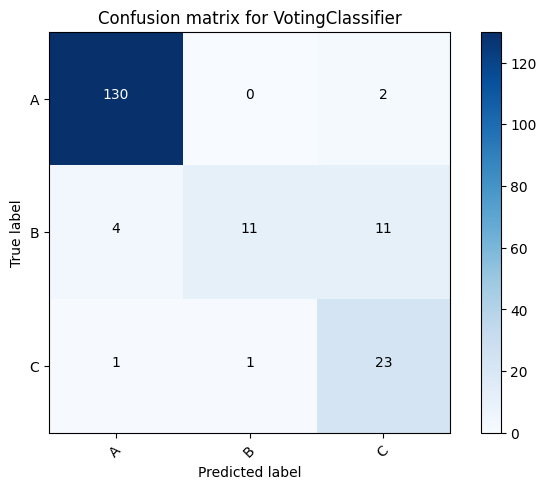
\includegraphics{transformer-paper4_files/figure-pdf/cell-9-output-2.png}

}

\end{figure}

\hypertarget{second-case-training-using-all-of-the-data-from-dataset-a}{%
\section{Second case: Training using all of the data from Dataset
A}\label{second-case-training-using-all-of-the-data-from-dataset-a}}

So far we have used 75\% of Dataset A to train the data and 25\% to test
it. Here, we used all of the data from Dataset A to train, and then test
it on Dataset B.

\begin{Shaded}
\begin{Highlighting}[]
\ImportTok{from}\NormalTok{ sklearn.ensemble }\ImportTok{import}\NormalTok{ RandomForestClassifier}
\ImportTok{from}\NormalTok{ sklearn.ensemble }\ImportTok{import}\NormalTok{ VotingClassifier}
\ImportTok{from}\NormalTok{ sklearn.linear\_model }\ImportTok{import}\NormalTok{ LogisticRegression}
\ImportTok{from}\NormalTok{ sklearn.svm }\ImportTok{import}\NormalTok{ SVC}
\ImportTok{from}\NormalTok{ sklearn.neighbors }\ImportTok{import}\NormalTok{ KNeighborsClassifier}
\ImportTok{from}\NormalTok{ xgboost }\ImportTok{import}\NormalTok{ XGBClassifier}
\ImportTok{from}\NormalTok{ sklearn.neural\_network }\ImportTok{import}\NormalTok{ MLPClassifier}
\ImportTok{from}\NormalTok{ sklearn.naive\_bayes }\ImportTok{import}\NormalTok{ GaussianNB}
\ImportTok{from}\NormalTok{ sklearn.ensemble }\ImportTok{import}\NormalTok{ AdaBoostClassifier}

\NormalTok{lr\_clf }\OperatorTok{=}\NormalTok{ LogisticRegression(max\_iter}\OperatorTok{=}\DecValTok{10000}\NormalTok{)}
\NormalTok{svm\_clf }\OperatorTok{=}\NormalTok{ SVC(probability}\OperatorTok{=}\VariableTok{True}\NormalTok{)}
\NormalTok{knn\_clf }\OperatorTok{=}\NormalTok{ KNeighborsClassifier()}
\NormalTok{xgb\_clf }\OperatorTok{=}\NormalTok{ XGBClassifier(learning\_rate}\OperatorTok{=}\FloatTok{0.01}\NormalTok{, n\_estimators}\OperatorTok{=}\DecValTok{300}\NormalTok{, max\_depth}\OperatorTok{=}\DecValTok{3}\NormalTok{, subsample}\OperatorTok{=}\FloatTok{0.7}\NormalTok{)}
\NormalTok{mlp\_clf }\OperatorTok{=}\NormalTok{ MLPClassifier(hidden\_layer\_sizes}\OperatorTok{=}\NormalTok{(}\DecValTok{100}\NormalTok{,), max\_iter}\OperatorTok{=}\DecValTok{1000}\NormalTok{)}
\NormalTok{nb\_clf }\OperatorTok{=}\NormalTok{ GaussianNB()}
\CommentTok{\#ada\_clf = AdaBoostClassifier(n\_estimators=50, learning\_rate=0.003)}

\NormalTok{voting\_clf }\OperatorTok{=}\NormalTok{ VotingClassifier(}
\NormalTok{  estimators}\OperatorTok{=}\NormalTok{[}\CommentTok{\#(\textquotesingle{}nn\textquotesingle{}, mlp\_clf),}
              \CommentTok{\#(\textquotesingle{}svc\textquotesingle{}, svm\_clf),}
\NormalTok{              (}\StringTok{\textquotesingle{}knn\textquotesingle{}}\NormalTok{, knn\_clf), }\CommentTok{\#(\textquotesingle{}ada\textquotesingle{}, ada\_clf),(\textquotesingle{}nb\textquotesingle{}, nb\_clf)}
\NormalTok{              (}\StringTok{\textquotesingle{}xgb\textquotesingle{}}\NormalTok{, xgb\_clf), (}\StringTok{\textquotesingle{}lr\textquotesingle{}}\NormalTok{, lr\_clf)],}
\NormalTok{  voting}\OperatorTok{=}\StringTok{\textquotesingle{}hard\textquotesingle{}}\NormalTok{)}
\NormalTok{voting\_clf.fit(X\_A, y\_A)}
\end{Highlighting}
\end{Shaded}

\begin{verbatim}
VotingClassifier(estimators=[('knn', KNeighborsClassifier()),
                             ('xgb',
                              XGBClassifier(base_score=None, booster=None,
                                            callbacks=None,
                                            colsample_bylevel=None,
                                            colsample_bynode=None,
                                            colsample_bytree=None,
                                            early_stopping_rounds=None,
                                            enable_categorical=False,
                                            eval_metric=None,
                                            feature_types=None, gamma=None,
                                            gpu_id=None, grow_policy=None,
                                            importance_type=None,
                                            interaction_constraints=None,
                                            learning_rate=0.01, max_bin=None,
                                            max_cat_threshold=None,
                                            max_cat_to_onehot=None,
                                            max_delta_step=None, max_depth=3,
                                            max_leaves=None,
                                            min_child_weight=None, missing=nan,
                                            monotone_constraints=None,
                                            n_estimators=300, n_jobs=None,
                                            num_parallel_tree=None,
                                            predictor=None, random_state=None, ...)),
                             ('lr', LogisticRegression(max_iter=10000))])
\end{verbatim}

\begin{Shaded}
\begin{Highlighting}[]
\ImportTok{from}\NormalTok{ sklearn.metrics }\ImportTok{import}\NormalTok{ accuracy\_score}

\ControlFlowTok{for}\NormalTok{ clf }\KeywordTok{in}\NormalTok{ (}\CommentTok{\#mlp\_clf, svm\_clf, \#ada\_clf,}
\NormalTok{            knn\_clf, xgb\_clf, lr\_clf, }\CommentTok{\#nb\_clf,}
\NormalTok{            voting\_clf):}
\NormalTok{    clf.fit(X\_A, y\_A)}
\NormalTok{    y\_pred\_B }\OperatorTok{=}\NormalTok{ clf.predict(X\_B)}
    \BuiltInTok{print}\NormalTok{(clf.\_\_class\_\_.}\VariableTok{\_\_name\_\_} \OperatorTok{+} \StringTok{" for dataset B:"}\NormalTok{, accuracy\_score(y\_B, y\_pred\_B))}
\end{Highlighting}
\end{Shaded}

\begin{verbatim}
KNeighborsClassifier for dataset B: 0.8379204892966361
XGBClassifier for dataset B: 0.7706422018348624
LogisticRegression for dataset B: 0.8134556574923547
VotingClassifier for dataset B: 0.8256880733944955
\end{verbatim}

The code below is a function to visualize the confusion matrix

\begin{Shaded}
\begin{Highlighting}[]
\ImportTok{from}\NormalTok{ sklearn.metrics }\ImportTok{import}\NormalTok{ confusion\_matrix}
\ImportTok{import}\NormalTok{ itertools}
\KeywordTok{def}\NormalTok{ plot\_confusion\_matrix(cm, classes, normalize}\OperatorTok{=}\VariableTok{False}\NormalTok{, cmap}\OperatorTok{=}\NormalTok{plt.cm.Blues, title}\OperatorTok{=}\StringTok{\textquotesingle{}Confusion matrix\textquotesingle{}}\NormalTok{):}
    \ControlFlowTok{if}\NormalTok{ normalize:}
\NormalTok{        cm }\OperatorTok{=}\NormalTok{ cm.astype(}\StringTok{\textquotesingle{}float\textquotesingle{}}\NormalTok{) }\OperatorTok{/}\NormalTok{ cm.}\BuiltInTok{sum}\NormalTok{(axis}\OperatorTok{=}\DecValTok{1}\NormalTok{)[:, np.newaxis]}
        \BuiltInTok{print}\NormalTok{(}\StringTok{"Normalized confusion matrix"}\NormalTok{)}
    \ControlFlowTok{else}\NormalTok{:}
        \BuiltInTok{print}\NormalTok{(}\StringTok{\textquotesingle{}Confusion matrix, without normalization\textquotesingle{}}\NormalTok{)}
    \BuiltInTok{print}\NormalTok{(cm)}

\NormalTok{    plt.imshow(cm, interpolation}\OperatorTok{=}\StringTok{\textquotesingle{}nearest\textquotesingle{}}\NormalTok{, cmap}\OperatorTok{=}\NormalTok{cmap)}
\NormalTok{    plt.title(title)}
\NormalTok{    plt.colorbar()}
\NormalTok{    tick\_marks }\OperatorTok{=}\NormalTok{ np.arange(}\BuiltInTok{len}\NormalTok{(classes))}
\NormalTok{    plt.xticks(tick\_marks, classes, rotation}\OperatorTok{=}\DecValTok{45}\NormalTok{)}
\NormalTok{    plt.yticks(tick\_marks, classes)}

\NormalTok{    fmt }\OperatorTok{=} \StringTok{\textquotesingle{}.2f\textquotesingle{}} \ControlFlowTok{if}\NormalTok{ normalize }\ControlFlowTok{else} \StringTok{\textquotesingle{}d\textquotesingle{}}
\NormalTok{    thresh }\OperatorTok{=}\NormalTok{ cm.}\BuiltInTok{max}\NormalTok{() }\OperatorTok{/} \FloatTok{2.}
    \ControlFlowTok{for}\NormalTok{ i, j }\KeywordTok{in}\NormalTok{ itertools.product(}\BuiltInTok{range}\NormalTok{(cm.shape[}\DecValTok{0}\NormalTok{]), }\BuiltInTok{range}\NormalTok{(cm.shape[}\DecValTok{1}\NormalTok{])):}
\NormalTok{        plt.text(j, i, }\BuiltInTok{format}\NormalTok{(cm[i, j], fmt),}
\NormalTok{                 horizontalalignment}\OperatorTok{=}\StringTok{"center"}\NormalTok{,}
\NormalTok{                 color}\OperatorTok{=}\StringTok{"white"} \ControlFlowTok{if}\NormalTok{ cm[i, j] }\OperatorTok{\textgreater{}}\NormalTok{ thresh }\ControlFlowTok{else} \StringTok{"black"}\NormalTok{)}

\NormalTok{    plt.tight\_layout()}
\NormalTok{    plt.ylabel(}\StringTok{\textquotesingle{}True label\textquotesingle{}}\NormalTok{)}
\NormalTok{    plt.xlabel(}\StringTok{\textquotesingle{}Predicted label\textquotesingle{}}\NormalTok{)}
\end{Highlighting}
\end{Shaded}

Confusion Matrix:

\begin{Shaded}
\begin{Highlighting}[]
\NormalTok{class\_names }\OperatorTok{=}\NormalTok{ [}\StringTok{\textquotesingle{}A\textquotesingle{}}\NormalTok{, }\StringTok{\textquotesingle{}B\textquotesingle{}}\NormalTok{, }\StringTok{\textquotesingle{}C\textquotesingle{}}\NormalTok{]}

\ControlFlowTok{for}\NormalTok{ clf }\KeywordTok{in}\NormalTok{ (}\CommentTok{\#mlp\_clf, svm\_clf, \#ada\_clf,}
\NormalTok{            knn\_clf, xgb\_clf, lr\_clf, }\CommentTok{\#nb\_clf,}
\NormalTok{            voting\_clf):}
\NormalTok{    clf.fit(X\_A, y\_A)}
\NormalTok{    y\_pred\_B }\OperatorTok{=}\NormalTok{ clf.predict(X\_B)}
\NormalTok{    cnf\_matrix }\OperatorTok{=}\NormalTok{ confusion\_matrix(y\_B, y\_pred\_B)}
\NormalTok{    np.set\_printoptions(precision}\OperatorTok{=}\DecValTok{2}\NormalTok{)}
\NormalTok{    plt.figure()}
\NormalTok{    plot\_confusion\_matrix(cnf\_matrix, classes}\OperatorTok{=}\NormalTok{class\_names,}
\NormalTok{                          title}\OperatorTok{=}\StringTok{\textquotesingle{}Confusion matrix for \textquotesingle{}} \OperatorTok{+}\NormalTok{ clf.\_\_class\_\_.}\VariableTok{\_\_name\_\_}\NormalTok{)}
\NormalTok{    plt.show()}
\end{Highlighting}
\end{Shaded}

\begin{verbatim}
Confusion matrix, without normalization
[[245   8   4]
 [ 11  11  18]
 [  8   4  18]]
\end{verbatim}

\begin{figure}[H]

{\centering 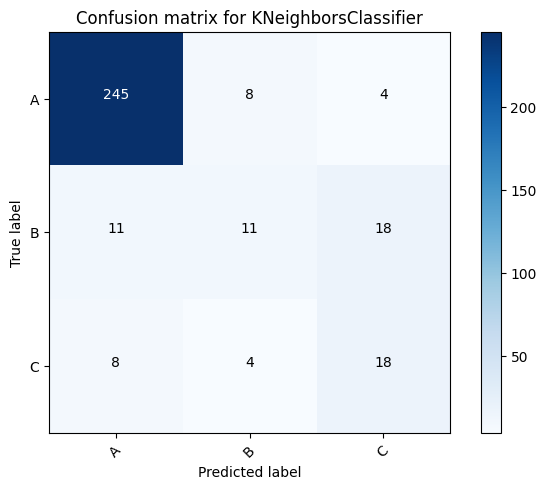
\includegraphics{transformer-paper4_files/figure-pdf/cell-13-output-2.png}

}

\end{figure}

\begin{verbatim}
Confusion matrix, without normalization
[[222  20  15]
 [  6   3  31]
 [  3   0  27]]
\end{verbatim}

\begin{figure}[H]

{\centering 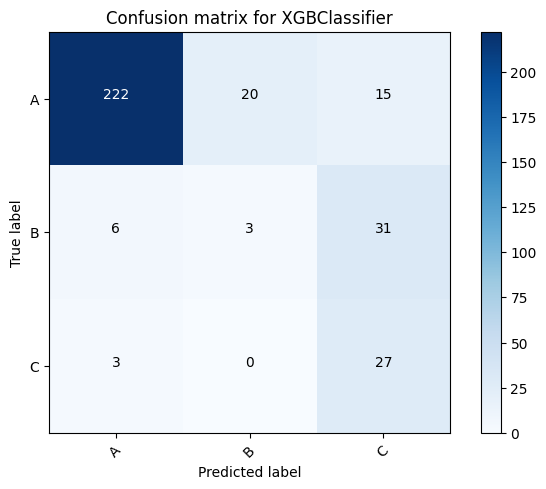
\includegraphics{transformer-paper4_files/figure-pdf/cell-13-output-4.png}

}

\end{figure}

\begin{verbatim}
Confusion matrix, without normalization
[[235  17   5]
 [ 10   7  23]
 [  5   1  24]]
\end{verbatim}

\begin{figure}[H]

{\centering 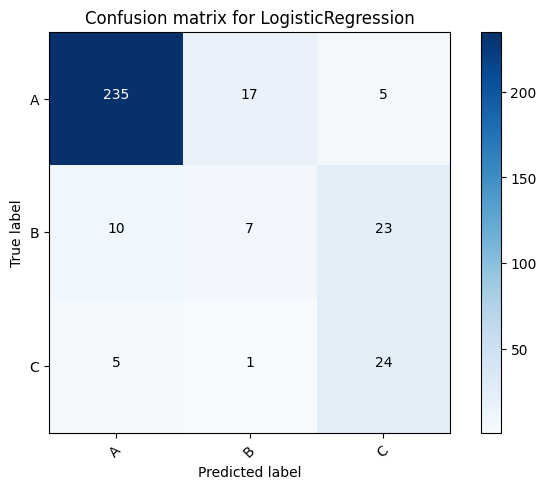
\includegraphics{transformer-paper4_files/figure-pdf/cell-13-output-6.png}

}

\end{figure}

\begin{verbatim}
Confusion matrix, without normalization
[[242  10   5]
 [ 10   3  27]
 [  5   0  25]]
\end{verbatim}

\begin{figure}[H]

{\centering 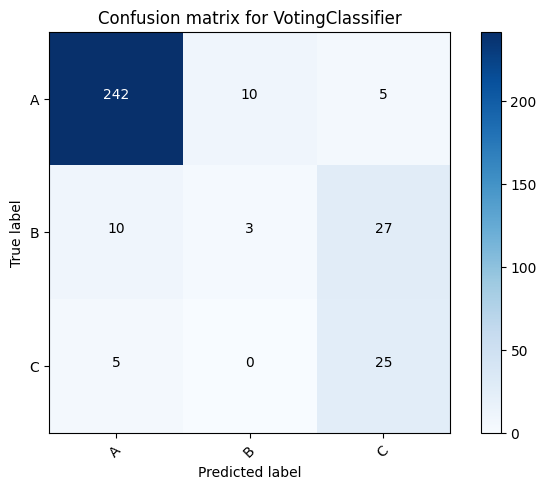
\includegraphics{transformer-paper4_files/figure-pdf/cell-13-output-8.png}

}

\end{figure}

\begin{Shaded}
\begin{Highlighting}[]
\NormalTok{class\_names }\OperatorTok{=}\NormalTok{ [}\StringTok{\textquotesingle{}A\textquotesingle{}}\NormalTok{, }\StringTok{\textquotesingle{}B\textquotesingle{}}\NormalTok{, }\StringTok{\textquotesingle{}C\textquotesingle{}}\NormalTok{]}
\NormalTok{voting\_clf.fit(X\_A, y\_A)}
\NormalTok{y\_pred\_B }\OperatorTok{=}\NormalTok{ voting\_clf.predict(X\_B)}
\NormalTok{cnf\_matrix }\OperatorTok{=}\NormalTok{ confusion\_matrix(y\_B, y\_pred\_B)}
\NormalTok{np.set\_printoptions(precision}\OperatorTok{=}\DecValTok{2}\NormalTok{)}
\NormalTok{plt.figure()}
\NormalTok{plot\_confusion\_matrix(cnf\_matrix, classes}\OperatorTok{=}\NormalTok{class\_names,}
\NormalTok{                      title}\OperatorTok{=}\StringTok{\textquotesingle{}Confusion matrix for \textquotesingle{}} \OperatorTok{+}\NormalTok{ clf.\_\_class\_\_.}\VariableTok{\_\_name\_\_}\NormalTok{)}
\NormalTok{plt.show()}
\end{Highlighting}
\end{Shaded}

\begin{verbatim}
Confusion matrix, without normalization
[[242  10   5]
 [ 10   3  27]
 [  5   0  25]]
\end{verbatim}

\begin{figure}[H]

{\centering 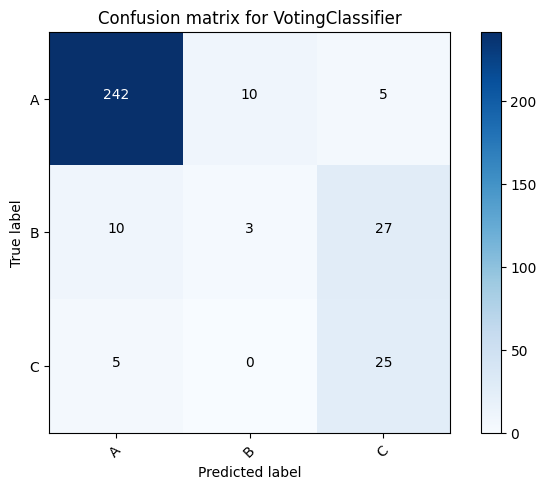
\includegraphics{transformer-paper4_files/figure-pdf/cell-14-output-2.png}

}

\end{figure}



\end{document}
